\documentclass[10pt,conference,onecolumn,compsoc]{IEEEtran}


\usepackage{hyperref}
\usepackage{enumitem}
\setlist[itemize]{leftmargin=3 cm}
\setlist[enumerate]{leftmargin=3cm}



% *** CITATION PACKAGES ***
%
\ifCLASSOPTIONcompsoc
  % IEEE Computer Society needs nocompress option
  % requires cite.sty v4.0 or later (November 2003)
  \usepackage[nocompress]{cite}
\else
  % normal IEEE
  \usepackage{cite}
\fi

% *** GRAPHICS RELATED PACKAGES ***
%
\ifCLASSINFOpdf
   \usepackage[pdftex]{graphicx}
  % declare the path(s) where your graphic files are
  % \graphicspath{{../pdf/}{../jpeg/}}
  % and their extensions so you won't have to specify these with
  % every instance of \includegraphics
  % \DeclareGraphicsExtensions{.pdf,.jpeg,.png}
\else
  % or other class option (dvipsone, dvipdf, if not using dvips). graphicx
  % will default to the driver specified in the system graphics.cfg if no
  % driver is specified.
  % \usepackage[dvips]{graphicx}
  % declare the path(s) where your graphic files are
  % \graphicspath{{../eps/}}
  % and their extensions so you won't have to specify these with
  % every instance of \includegraphics
  % \DeclareGraphicsExtensions{.eps}
\fi




% correct bad hyphenation here
\hyphenation{op-tical net-works semi-conduc-tor}


\begin{document}

\title{SBI Managment system}


\author{Kevin Patel\\Jeff Jordan
}

\IEEEtitleabstractindextext{%
\begin{abstract}
SBI Management System, named after the flagship Stone Brook Inn, is a program for use in the commercial Hospitality business in order to easily navigate the processes of booking, reserving, and maintaining rooms in an effective way to alleviate stresses of overbooking and unavailable rooms within businesses. 

\end{abstract}
}
\maketitle

\IEEEdisplaynontitleabstractindextext

\IEEEpeerreviewmaketitle



\section{Introduction}

The purpose of the SBI Management system is to remove the clerical errors of record keeping by hand and to cut down on the potential mistakes that could happen with note taking with rotating cast of
managerial staff and employees. It is designed around the idea of condensing and centralizing all reservation and booking information into one simple, easy-to-use application in order to remove the stress of record keeping and room tracking. 

On the backend, it will keep track of non-confidential customer information. The purpose of this is to implement features such as a customer rewards program, discounts, personalized service, etc. In the future, it will implement encryption for payment information. 

\subsection{Background}
A member of our group's family owns a hotel. This project is being designed with the needs of an actual hotel business in mind. The design will be centered around a simple GUI to quickly assign rooms and check availability. 

While the primary purpose of the project is for the Stone Brook Inn, we will design it to be implemented by any local small hotel or motel. The idea is to keep the functionality universal while making design edits simple and easy to understand. 

\subsection{Challenges}
Integrating legal and secure encryption for web payments will be the ultimate challenge for the project. 
Ensuring that the program doesn't allow for any booking of unavailable rooms will be a challenge since there will be a lot of test cases that might go unnoticed.
Designing a universal program that could be adjusted to fit any business model might present itself to be more challenging than we can currently foresee. 


\section{Scope}
The scope of this program will be extensive. It will handle guest checkins and checkouts, it will feature an intuitive and powerful interface, it will be adjustable to any hotel, it will ensure no overbooking issues arise, will keep track of customer rewards points, and lastly, feature a cross-shift note system. 

\subsection{Requirements}
The main requirement is a visual of the hotel's rooms and what it available, as well as what's already reserved. Another requirement is the functionality to take in a customer's information and turn a vacant room into a reserved room. 

\subsubsection{Functional}
\begin{itemize}
\item Visual map of the rooms.
\item Color coding of availability.
\item User information field.
\item Notes
\end{itemize}

\subsubsection{Non-Functional}
\begin{itemize}
\item Security -- The note system should be hidden until clicked.
\end{itemize}

\subsection{Use Cases}

\begin{table}
\centering
\begin{tabular}{|c|c|c|c|c|}
\hline
1 & Release occupancy\\
\hline \hline
2 & Fill vacancy\\
\hline

\end{tabular}
\caption{Use Cases}
\label{tab:useCaseIndex}
\end{table}


\begin{itemize}
\item[Use Case Number:] 1
\item[Use Case Name:] Booking and Maintaining Rooms
\item[Description:] Administrators at motel and hotel businesses will be able to block rooms once they are booked by customers or repairs/cleaning needs to take place.

\item[Use Case Number:] 2
\item[Use Case Name:] Reservations
\item[Description:] Interact with a calender in order to properly plan out and schedule rooms to be booked and blocked to prevent overbooking.
\end{itemize}

\subsection{Interface Mockups}
\begin{figure}[ht!]
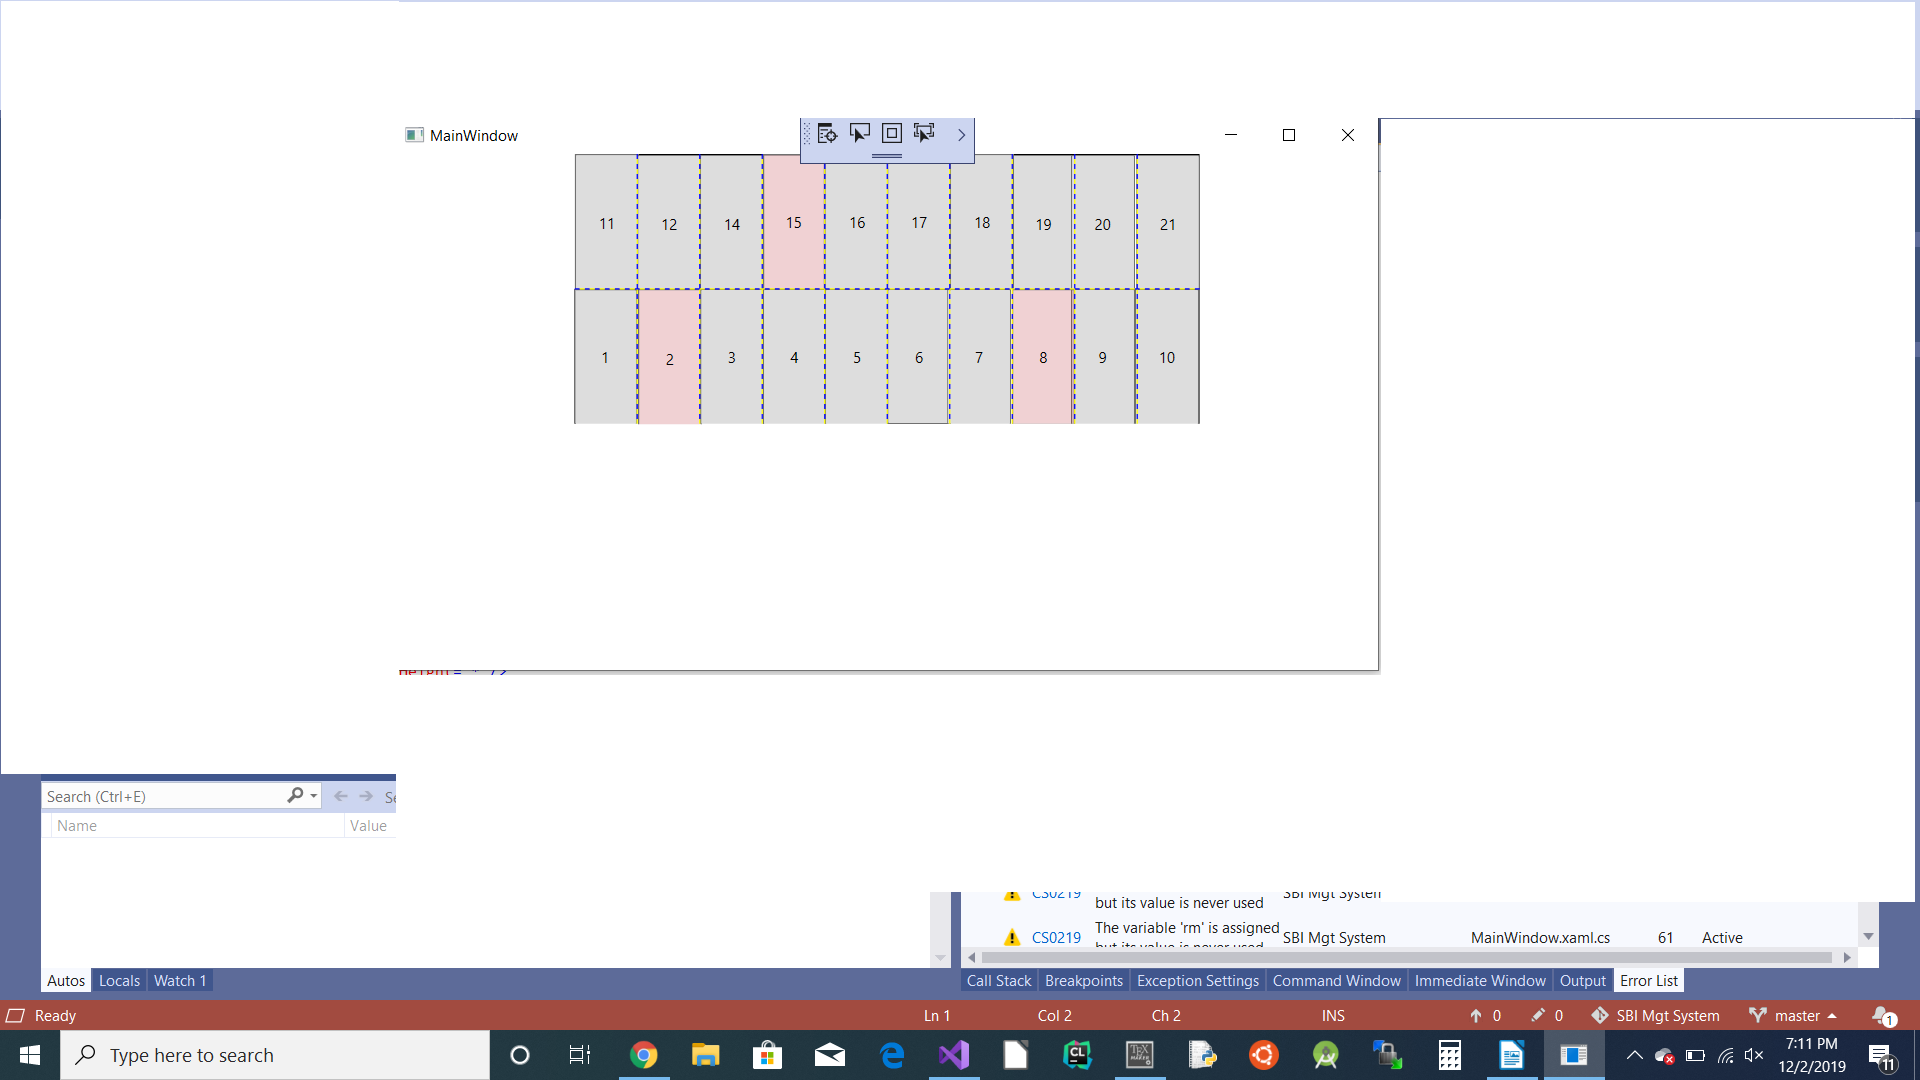
\includegraphics[height=250px, width=350px]{GUI.png}
\caption{Main window of the program}
\label{Interface}
\end{figure}


\section{Project Timeline}
A large portion of our time spent on this project was on design. To be honest, too much time was spent on the design. It wasn't until, two months in, that we started the actual coding of the project, that the design fell into place all on its own. 

Within two days, we had moved past the design and delved into the requirements. First came the buttons themselves. Each button needed to act separately from the others, so it took over a month to manage everything that needed to happen upon button clicks. Some of these issues were color changes, form population, and a note system.

This last month has been committed to polishing and trying to learn a database. We eventually gave up on the database and will store all information as notes.

\section{Project Structure}
By the project's culmination, it turned into a day to day system to manage availability of rooms for the hotel. It has a working GUI, and upon filling in the information about reservation, it will mark the room unavailable with a color change. There is another button that will change it back to available. 

All information is stored in a display box for notes, in lieu of a database. We realized there is no point since they have no rewards system in place at the hotel yet. 

\subsection{UML Outline}





\subsection{Design Patterns Used}
The decorator design pattern was used on buttons. Upon another button's clicking, a separate button will change color. 


\section{Results}
This section will start out a little vague, but it should grow as your project evolves.  With each deliverable you hand in, give me a final summary of where your project stands.  By the end, this should be a reflective section discussing how many of your original goals you managed to attain/how many desired use cases you implemented/how many extra features you added.

\subsection{Future Work}
Future work will include tweaking as it's used in the field. There will need to be a save system in case of recovery upon crash. If the hotel ever adds a reward system, there will need to be a database implemented. 

\begin{thebibliography}{1}

\bibitem{IEEEhowto:kopka}
H.~Kopka and P.~W. Daly, \emph{A Guide to \LaTeX}, 3rd~ed.\hskip 1em plus
  0.5em minus 0.4em\relax Harlow, England: Addison-Wesley, 1999.

\end{thebibliography}



\begin{IEEEbiography}{Michael Shell}
Biography text here.
\end{IEEEbiography}

% if you will not have a photo at all:
\begin{IEEEbiographynophoto}{John Doe}
Biography text here.
\end{IEEEbiographynophoto}

\begin{IEEEbiographynophoto}{Jane Doe}
Biography text here.
\end{IEEEbiographynophoto}


\end{document}